\ifx\allfiles\undefined
\documentclass[12pt, a4paper,oneside, UTF8]{ctexbook}
\usepackage[dvipsnames]{xcolor}
\usepackage{amsmath}   % 数学公式
\usepackage{amsthm}    % 定理环境
\usepackage{amssymb}   % 更多公式符号
\usepackage{graphicx}  % 插图
%\usepackage{mathrsfs}  % 数学字体
%\usepackage{newtxtext,newtxmath}
%\usepackage{arev}
\usepackage{kmath,kerkis}
\usepackage{newtxtext}
\usepackage{bbm}
\usepackage{enumitem}  % 列表
\usepackage{geometry}  % 页面调整
%\usepackage{unicode-math}
\usepackage[colorlinks,linkcolor=black]{hyperref}

\usepackage{wrapfig}


\usepackage{ulem}	   % 用于更多的下划线格式,
					   % \uline{}下划线,\uuline{}双下划线,\uwave{}下划波浪线,\sout{}中间删除线,\xout{}斜删除线
					   % \dashuline{}下划虚线,\dotuline{}文字底部加点


\graphicspath{ {flg/},{../flg/}, {config/}, {../config/} }  % 配置图形文件检索目录
\linespread{1.5} % 行高

% 页码设置
\geometry{top=25.4mm,bottom=25.4mm,left=20mm,right=20mm,headheight=2.17cm,headsep=4mm,footskip=12mm}

% 设置列表环境的上下间距
\setenumerate[1]{itemsep=5pt,partopsep=0pt,parsep=\parskip,topsep=5pt}
\setitemize[1]{itemsep=5pt,partopsep=0pt,parsep=\parskip,topsep=5pt}
\setdescription{itemsep=5pt,partopsep=0pt,parsep=\parskip,topsep=5pt}

% 定理环境
% ########## 定理环境 start ####################################
\theoremstyle{definition}
\newtheorem{defn}{\indent 定义}[section]

\newtheorem{lemma}{\indent 引理}[section]    % 引理 定理 推论 准则 共用一个编号计数
\newtheorem{thm}[lemma]{\indent 定理}
\newtheorem{corollary}[lemma]{\indent 推论}
\newtheorem{criterion}[lemma]{\indent 准则}

\newtheorem{proposition}{\indent 命题}[section]
\newtheorem{example}{\indent \color{SeaGreen}{例}}[section] % 绿色文字的 例 ,不需要就去除\color{SeaGreen}{}
\newtheorem*{rmk}{\indent \color{red}{注}}

% 两种方式定义中文的 证明 和 解 的环境:
% 缺点:\qedhere 命令将会失效【技术有限,暂时无法解决】
\renewenvironment{proof}{\par\textbf{证明.}\;}{\qed\par}
\newenvironment{solution}{\par{\textbf{解.}}\;}{\qed\par}

% 缺点:\bf 是过时命令,可以用 textb f等替代,但编译会有关于字体的警告,不过不影响使用【技术有限,暂时无法解决】
%\renewcommand{\proofname}{\indent\bf 证明}
%\newenvironment{solution}{\begin{proof}[\indent\bf 解]}{\end{proof}}
% ######### 定理环境 end  #####################################

% ↓↓↓↓↓↓↓↓↓↓↓↓↓↓↓↓↓ 以下是自定义的命令  ↓↓↓↓↓↓↓↓↓↓↓↓↓↓↓↓

% 用于调整表格的高度  使用 \hline\xrowht{25pt}
\newcommand{\xrowht}[2][0]{\addstackgap[.5\dimexpr#2\relax]{\vphantom{#1}}}

% 表格环境内长内容换行
\newcommand{\tabincell}[2]{\begin{tabular}{@{}#1@{}}#2\end{tabular}}

% 使用\linespread{1.5} 之后 cases 环境的行高也会改变,重新定义一个 ca 环境可以自动控制 cases 环境行高
\newenvironment{ca}[1][1]{\linespread{#1} \selectfont \begin{cases}}{\end{cases}}
% 和上面一样
\newenvironment{vx}[1][1]{\linespread{#1} \selectfont \begin{vmatrix}}{\end{vmatrix}}

\def\d{\textup{d}} % 直立体 d 用于微分符号 dx
\def\R{\mathbb{R}} % 实数域
\def\N{\mathbb{N}} % 自然数域
\def\C{\mathbb{C}} % 复数域
\def\Z{\mathbb{Z}} % 整数环
\def\Q{\mathbb{Q}} % 有理数域
\newcommand{\bs}[1]{\boldsymbol{#1}}    % 加粗,常用于向量
\newcommand{\ora}[1]{\overrightarrow{#1}} % 向量

% 数学 平行 符号
\newcommand{\pll}{\kern 0.56em/\kern -0.8em /\kern 0.56em}

% 用于空行\myspace{1} 表示空一行 填 2 表示空两行  
\newcommand{\myspace}[1]{\par\vspace{#1\baselineskip}}

%s.t. 用\st就能打出s.t.
\DeclareMathOperator{\st}{s.t.}

%罗马数字 \rmnum{}是小写罗马数字, \Rmnum{}是大写罗马数字
\makeatletter
\newcommand{\rmnum}[1]{\romannumeral #1}
\newcommand{\Rmnum}[1]{\expandafter@slowromancap\romannumeral #1@}
\makeatother
\begin{document}
	% \title{{\Huge{\textbf{$Real \,\, Analysis$}}}\\
		\Large{\textbf{$Measure \,\, Theory , \,\, Integration , \,\, \& \,\, Hilbert \,\, Spaces$}}\footnote{参考书籍:\\
			\hspace*{4em} \textbf{《$Real \,\, Analysis -- Measure \,\, Theroy, \,\, Integration, \,\, \& \,\, Hilbert \,\, Spaces$》--- $Elias \,\, M. \,\, Stein$} \\
			\hspace*{4em} \textbf{《$Real \,\, Analysis -- Modern \,\, Techniques \,\, and \,\, Their \,\, Applications$》--- $Gerald \,\, B. \,\, Folland$}}}
\author{$-TW-$}
\date{\today}
\maketitle                   % 在单独的标题页上生成一个标题

\thispagestyle{empty}        % 前言页面不使用页码
\begin{center}
	\Huge\textbf{序}
\end{center}


\vspace*{3em}
\begin{center}
	\large{\textbf{天道几何,万品流形先自守;}}\\
	
	\large{\textbf{变分无限,孤心测度有同伦。}}
\end{center}

\vspace*{3em}
\begin{flushright}
	\begin{tabular}{c}
		\today \\ \small{\textbf{长夜伴浪破晓梦,梦晓破浪伴夜长}}
	\end{tabular}
\end{flushright}


\newpage                      % 新的一页
\pagestyle{plain}             % 设置页眉和页脚的排版方式(plain:页眉是空的,页脚只包含一个居中的页码)
\setcounter{page}{1}          % 重新定义页码从第一页开始
\pagenumbering{Roman}         % 使用大写的罗马数字作为页码
\tableofcontents              % 生成目录

\newpage                      % 以下是正文
\pagestyle{plain}
\setcounter{page}{1}          % 使用阿拉伯数字作为页码
\pagenumbering{arabic}
\setcounter{chapter}{0}    % 设置 -1 可作为第零章绪论从第零章开始 
	\else
	\fi
	%  ############################ 正文部分
\chapter{$Differentiation \,\, and \,\, Integration$}
\paragraph{\textbf{Motivation}}
	在\textbf{Riemann积分}的框架下,我们知道\textbf{积分}和\textbf{微分}可以视作一对互逆的运算. 而在这一章,我们将在全新的\textbf{Lebesgue测度}的框架下重新审视\textbf{积分}和\textbf{微分}之间的关系.
	
	\vspace{1em}
	下面先来描述一下想要解决的问题.
	\begin{itemize}
		\item Let $f \in \mathcal{L}^{1}(\R^d)$. 对于\textbf{变上限积分}$F(x) = \int_{a}^{x}{f(y) dy}$,我们知道根据\textbf{Riemann积分下的微积分基本定理},对$F$求导就会回到被积函数$f$ 本身. 那么我们就会好奇:
		
		\vspace{1em}
		
		\begin{itemize}
			\item 在\textbf{Lebesgue积分}的框架下,这个结论是否还成立?
			
			\item 如果成立的话,又对哪些$x$成立呢?
		\end{itemize}
	
		\vspace{1em}
		
		此时回顾求导的定义,即对于差商 (此处改写为更具一般性的符号$I = (x , x + h)$)
		\begin{align}
			\frac{F(x + h) - F(x)}{h} 
			= \frac{1}{h} \int_{x}^{x + h}{f(y) dy} 
			= \frac{1}{\left| I \right|} \int_{I}{f(y) dy}
		\end{align}
		对差商中的增量$h \to 0$,即得到\textbf{导数}的定义. 那么我们的问题就转化为了
		\begin{align}
			\lim_{\substack{\left| I \right| \to 0 \\ I \ni x}}{\frac{1}{\left| I \right|} \int_{I}{f(y) dy}}
			= f(x) 
			\,\,\,\, \text{holds for which $x$?}
		\end{align}
	
		\vspace{1em}
		
		更一般地,将上述问题从一维实直线$\R$ 推广至$\R^d$ 空间上,将区间$I$ 用开球$B$ 替换,得
		\begin{align}
			\lim_{\substack{m(B) \to 0 \\ B \ni x}}{\frac{1}{m(B)} \int_{B}{f(y) dy}}
			= f(x)
			\,\,\,\, \text{holds for which $x$?}
		\end{align}
	
		\vspace{1em}
		
		\begin{rmk}
			\begin{itemize}
				\item 此处看似是随着开球$B$的测度减小,$x \in B$ 在跟着$B$ ``跑",但实际上则相反:
				\begin{center}
					对于每个固定的$x$,让包含着$x$ 的球$B \ni x$ 不断减小其测度,最后取极限 
				\end{center}	
				而这也就是此处极限条件写为``$B \ni x$" 而非``$x \in B$" 的原因,逻辑更清晰.
				
				\vspace{1em}
				
				\item 事实上该结论对于\textbf{几乎处处的$x$} 都成立 (若$f$ \textbf{Lebesgue可积}),这就是后面要讲的\textbf{Lebesgue微分定理}.
			\end{itemize}
		\end{rmk}
	\end{itemize}
	
\newpage
\section{$Hardy-Littlewood$ 极大函数 (非球心)}
\paragraph{定义}
	下面我们给出\textbf{Hardy-Littlewood 极大函数}的定义.
	\begin{defn}\label{def 4.1.1}
		If $f \in \mathcal{L}^{1}(\R^d)$, we define its \underline{\textcolor{blue}{\textbf{maximal function}}} $Mf$ by
		\begin{align}
			Mf(x) = \sup_{B \ni x}{\frac{1}{m(B)} \int_{B}{\left| f(y) \right| dy}}
		\end{align}
	
		\vspace{1em}
		\begin{rmk}
			我们目前并不知道球面测度的具体数值与计算方法,但事实上我们也并不需要知道其具体数值,具体表现在: \\
			设$\R^d$ 中单位球$B(0 , 1)$ 的测度为$m(B(0 , 1)) = v_d$. $\forall B(x , r) \subset \R^d$,根据\textbf{Lebesgue测度的平移不变性和伸缩变换公式 (Prop \ref{prop 3.7.1})}
			\begin{center}
				$B(0 , r) = r B(0 , 1) \,\, \Rightarrow \,\, m(B(x , r)) = m(B(0 , r)) = r^d m(B(0 , 1)) = r^d v_d$
			\end{center}
		\end{rmk}
	\end{defn}

\vspace{2em}
\paragraph{性质}
	下面来说明\textbf{Hardy-Littlewood 极大函数}的三条\textbf{性质}.
	\begin{proposition}\label{prop 4.1.1}
		Suppose $f \in \mathcal{L}^{1}(\R^d)$. Then:
		\begin{enumerate}
			\item[(\rmnum{1})]$Mf$ is measurable.
			
			\item[(\rmnum{2})]$Mf(x) < \infty$ for a.e. $x$.
			
			\item[(\rmnum{3})]\textbf{weak-type inequality}. \\
			$Mf$ satisfies
			\begin{align}
				m\left( \left\{ x \in \R^d \mid Mf(x) > \alpha \right\} \right) 
				\leq \frac{A}{\alpha} \,\, \Vert f \Vert_{\mathcal{L}^1} , \,\, \forall \alpha > 0
			\end{align}
			where $A = 3^d$.
		\end{enumerate}
	
		\vspace{4em}
		\begin{proof}
			\begin{enumerate}
				\item [(\rmnum{1})]Let $E_\alpha = \{ x \in \R^d \mid Mf(x) > \alpha \}$. 下面证明$E_\alpha$ open. \\
				$\forall x \in E_\alpha$, by the \textbf{definition of $Mf$ (Def \ref{def 4.1.1})}, $\exists B_x \ni x$, $\st$
				\begin{align}
					\frac{1}{m(B_x)} \int_{B_x}{\left| f \right|} > \alpha
				\end{align}
				Then $\forall y \in B_x$, $B_x$ is also an open ball containing $y$, so we have $y \in E_\alpha$. i.e. $B_x \subset E_\alpha$. \\
				Therefore, $E_\alpha$ is open, specifically measurable for all $\alpha$. Then $Mf$ is measurable.
				
				\newpage
				
				\item[(\rmnum{2})]下面说明(\rmnum{3}) $\Rightarrow$ (\rmnum{2}): \\
				Let $E_\alpha = \{ x \in \R^d \mid Mf(x) > \alpha \}$. Then $E_n \searrow E = \{ x \in \R^d \mid Mf(x) = \infty \}$. \\
				Since $f \in \mathcal{L}^{1}(\R^d)$, $\Vert f \Vert_{\mathcal{L}^1}$ is finite. Then by \textbf{(\rmnum{3})}, $m(E_1) < \infty$. \\
				Then by \textbf{Thm \ref{thm 1.3.3}},
				\begin{align}
					m(E) = \lim_{n \to \infty}{m(E_n)} \leq \lim_{n \to \infty}{\frac{A}{n} \,\, \Vert f \Vert_{\mathcal{L}^1}} = 0
				\end{align}
				Therefore $m(E) = 0$. i.e. $Mf(x) < \infty$ for a.e. $x$.
				
				\vspace{6em}
				
				\item[(\rmnum{3})]在证明(\rmnum{3})之前,先来介绍\textbf{Vitali覆盖引理}.
				
				\vspace{2em}
				
				\begin{lemma}\label{lemma 4.1.1}
					\textbf{Vitali Covering Lemma (Elementary Version)}. \\
					Suppose $\mathcal{B} = \{ B_1 , B_2 , \cdots , B_N \}$, $B_i \subset \R^d$ are open balls, then there is a disjoint subcollection $B_{i_1} , \cdots , B_{i_k}$ that satisfies
					\begin{align}
						m\left( \bigcup_{l = 1}^{N}{B_l} \right) 
						\leq 3^d \sum_{j = 1}^{k}{m(B_{i_j})}
					\end{align}
					
					\vspace{1em}
					\begin{rmk}
						这是\textbf{Vitali覆盖引理}的\textbf{初等版本 (有限版本)},更一般的版本是对\textbf{一列}球结论成立.
					\end{rmk}
				
					\vspace{1em}
					\begin{proof}
						详见视频\href{https://www.bilibili.com/video/BV1FT411C7wM?p=31}{(非球心)Hardy-Littlewood极大函数} 23:10 (类似\textbf{贪心算法}的迭代步骤)
					\end{proof}
					
					\begin{figure}[thbp!]
						\centering
						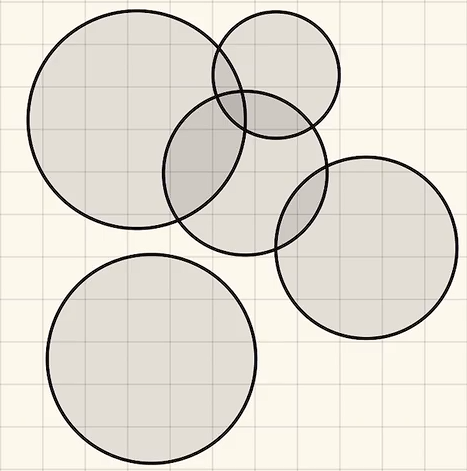
\includegraphics[width=0.25\linewidth]{figure/4.1.1-1}
						\caption{Lemma 4.1.1}
						\label{pic : 4.1.1-1} % 添加图像引用标签
					\end{figure}
				\end{lemma}
			
				\newpage
				
				下面继续来证明(\rmnum{3}): \\
				Fix $\alpha > 0$, $\forall x \in B_\alpha$, $\exists$ open ball $B_x$, $\st$
				\begin{align}
					\frac{1}{m(B_x)} \int_{B_x}{\left| f \right|} > \alpha
				\end{align}
				So we have $E_\alpha \subset \underset{x \in E_\alpha}{\bigcup}{B_x}$. \\
				Since $E_\alpha$ is measurable (by \textbf{(\rmnum{1})}), then by \textbf{Thm \ref{thm 1.3.4} (Lebesgue测度的内正则性)}, \\
				$\forall \epsilon > 0$, $\exists$ compact $K_\epsilon \subset E_\alpha$, $\st$
				\begin{center}
					$m(E_\alpha \backslash K_\epsilon) \leq \epsilon$
				\end{center}
				i.e.
				\begin{center}
					$m(E_\alpha) - m(K_\epsilon) \leq \epsilon$
				\end{center}
				Since $K_\epsilon$ is compact, $K_\epsilon \subset \underset{x \in K_\epsilon}{\bigcup}{B_x}$, there exists a subcollection $B_{x_1} , \cdots , B_{x_N}$, $\st$
				\begin{center}
					$K_\epsilon \subset \overset{N}{\underset{l = 1}{\bigcup}}{B_{x_l}}$
				\end{center}
				Then by \textbf{Vitali Covering Lemma (Lemma \ref{lemma 4.1.1})}, there exists a subcollection $B_{x_{i_1}} , \cdots , B_{x_{i_k}}$, $\st$
				\begin{center}
					$m\left( \overset{N}{\underset{l = 1}{\bigcup}}{B_{x_l}} \right) 
					\leq 3^d \overset{k}{\underset{j = 1}{\sum}}{m(B_{x_{i_j}})}$
				\end{center}
				Therefore
				\begin{align}
					m(K_\epsilon) 
					\leq m\left( \bigcup_{l = 1}^{N}{B_{x_l}} \right)
					&\leq 3^d \sum_{j = 1}^{k}{m(B_{x_{i_j}})} \\
					&= \frac{3^d}{\alpha} \sum_{j = 1}^{k}{\alpha \cdot m(B_{x_{i_j}})} \\
					&\leq \frac{3^d}{\alpha} \int_{\bigcup_{j = 1}^{k}{B_{x_{i_j}}}}{\left| f \right|} \\
					&\leq \frac{3^d}{\alpha} \int_{\R^d}{\left| f \right|} \\
					&= \frac{3^d}{\alpha} \,\, \Vert f \Vert_{\mathcal{L}^1}
				\end{align}
				Then
				\begin{align}
					m(E_\alpha) 
					\leq m(K_\epsilon) + \epsilon 
					\leq \frac{A}{\alpha} \,\, \Vert f \Vert_{\mathcal{L}^1} + \epsilon
				\end{align}
				where $A = 3^d$, $\epsilon > 0$. \\
				Since $\epsilon$ is arbitrary, let $\epsilon \to 0$, we have
				\begin{align}
					m(E_\alpha) \leq \frac{A}{\alpha} \,\, \Vert f \Vert_{\mathcal{L}^1} , \,\, A = 3^d , \,\, \forall \alpha > 0
				\end{align}
			\end{enumerate}
		\end{proof}
	\end{proposition}

\newpage
\section{$Lebesgue$ 微分定理 (非球心)}
	\begin{center}
		在这一节我们将利用\textbf{Hardy-Littlewood极大函数}来证明\textbf{Lebesgue微分定理}.
	\end{center}
	
\subsection{$Chebyshev's \,\, Inequality$}
	在此之前,我们先来证明一个非常有用的不等式,即\textbf{切比雪夫不等式}.
	\begin{thm}\label{thm 4.2.1}
		\textbf{Chebyshev's Inequality}. \\
		If $g \in \mathcal{L}^{1}(\R^d)$, then
		\begin{align}
			m\left( \left\{ x \in \R^d \mid \left| g(x) \right| > \alpha \right\} \right)
			\leq \frac{1}{\alpha} \,\, \Vert g \Vert_{\mathcal{L}^1} , \,\, \forall \alpha > 0
		\end{align}
		
		\vspace{4em}
		\begin{proof}
			Let $E_\alpha = \{ x \in \R^d \mid \left| g(x) \right| > \alpha \}$. Then
			\begin{align}
				\Vert g \Vert_{\mathcal{L}^1}
				= \int_{\R^d}{\left| g \right|}
				\geq \int_{E_\alpha}{\left| g \right|}
				\geq \int_{E_\alpha}{\alpha}
				= \alpha \cdot m(E_\alpha)
			\end{align}
		\end{proof}
	\end{thm}

\newpage
\subsection{$The \,\, Lebesgue \,\, Differentiation \,\, Theorem$}
	下面我们就来给出\textbf{Lebesgue微分定理}.
	\begin{thm}\label{thm 4.2.2}
		If $f \in \mathcal{L}^{1}(\R^d)$, then
		\begin{align}
			\lim_{\substack{m(B) \to 0 \\ B \ni x}}{\frac{1}{m(B)} \int_{B}{f(y) dy}} = f(x) \,\,\,\, for \,\, a.e. \,\, x
		\end{align}
		
		\vspace{2em}
		\begin{rmk}
			\begin{itemize}
				\item \textbf{Lebesgue微分定理}说明了对于\textbf{几乎处处的$x$},当包含$x$ 的球体$B$ 的测度趋于0时,$f$ 在球体$B$ 上积分的平均值就会收敛到$f(x)$.
				
				\vspace{2em}
				
				\item 定理左侧实际上是关于集合$B$ 的函数的一个极限过程,用$\epsilon-\delta$语言叙述如下:\\
				$\forall \epsilon > 0$, $\exists \delta> 0$, $\st$ for all $B \ni x$ and $m(B) < \delta$, we have
				\begin{align}
					\left| \frac{1}{m(B)} \int_{B}{f(y) dy} - f(x) \right| \leq \epsilon
				\end{align}
			
				\vspace{2em}
				
				\item 要证明该定理,首先需要说明等式左侧\textbf{极限的存在性},但这并不好说明. 为了跳过说明其存在性的问题,我们需要引入类似\textbf{``上极限"}的函数,即: \\
				If suffices to show
				\begin{align}
					\lim_{\delta \to 0}{\sup_{\substack{m(B) < \delta \\ B \ni x}}{\left| \frac{1}{m(B)} \int_{B}{f(y) dy} - f(x) \right|}} = 0 \,\,\,\, for \,\, a.e. \,\, x
				\end{align}
				由于极限内的函数随着$\delta$ 递减而单调递减,又存在下界$0$,因此在$\delta = 0$ 处必存在右极限. 这样就跳过了原极限是否存在的问题.
				
				\vspace{2em}
				
				\item 事实上此处极限\textbf{``怪异"}的本质原因在于开球$B$ 的选取的任意性,若将其定义为以$x$ 为球心, $r$ 为半径的球,则可直接令$r \to 0$ 变为正常的函数极限,即
				\begin{align}
					\lim_{r \to 0}{\frac{1}{m(B(x , r))} \int_{B(x , r)}{f(y) dy}} = f(x)
				\end{align}
				在下一节我们会从\textbf{Hardy-Littlewood极大函数}开始,以此方法重新说明\textbf{Lebesgue微分定理}.
			\end{itemize}
		\end{rmk}
	
		\newpage
		\begin{proof}
			Let 
			\begin{align}
				E_\alpha 
				= \left\{ x \in \R^d \mid \lim_{\delta \to 0}{\sup_{\substack{m(B) < \delta \\ B \ni x}}{\left| \frac{1}{m(B)} \int_{B}{f(y) dy} - f(x) \right| > 2 \alpha}} \right\}
			\end{align}
			Then we \textbf{WTS (want to show)}:
			\begin{center}
				$m(E_\alpha) = 0$, $\forall \alpha \geq 0$
			\end{center}
			
			\vspace{1em}
			
			Fix $\alpha \geq 0$. By \textbf{Thm \ref{thm 3.2.3}}, $C_{c}(\R^d)$ is dense in $\mathcal{L}^{1}(\R^d)$ (有紧支集的连续函数), then \\
			$\forall \epsilon > 0$, $\exists g \in C_{c}(\R^d)$, $\st$
			\begin{center}
				$\Vert f - g \Vert_{\mathcal{L}^1} < \epsilon$
			\end{center}
			Since $g$ is uniformly continuous, then $\exists \delta > 0$, $\st$
			\begin{align}
				\left| \frac{1}{m(B)} \int_{B}{g(y) dy} - g(x) \right| 
				\leq \frac{1}{m(B)} \int_{B}{\left| g(y) - g(x) \right| dy}
				< \frac{1}{m(B)} \int_{B}{\epsilon dy} 
				= \epsilon
			\end{align}
			for all $B \ni x$ and $m(B) < \delta$. 
			
			\vspace{2em}
			
			下面对$m(E_\alpha)$ 进行估计. $\forall x \in E_\alpha$,
			\begin{align}
				\left| \frac{1}{m(B)} \int_{B}{f(y) dy} - f(x) \right|
				\leq \left| \frac{1}{m(B)} \int_{B}{(f(y) - g(y)) dy} \right|
				+ \left| \frac{1}{m(B)} \int_{B}{g(y) dy} - g(x) \right|
				+ \left| g(x) - f(x) \right|
			\end{align}
			对上述不等式中的开球$B \ni x$ 取上确界$\sup$,得
			\begin{align}
				\sup_{B \ni x}{\left| \frac{1}{m(B)} \int_{B}{f(y) dy} - f(x) \right|}
				\leq \sup_{B \ni x}{\left| \frac{1}{m(B)} \int_{B}{(f(y) - g(y)) dy} \right|}
				+ \sup_{B \ni x}{\left| \frac{1}{m(B)} \int_{B}{g(y) dy} - g(x) \right|}
				+ \left| g(x) - f(x) \right|
			\end{align}
			再令$m(B) \to 0$,由于根据\textbf{式 (4.24)},
			\begin{align}
				\lim_{\delta \to 0}{\sup_{\substack{m(B) < \delta \\ B \ni x}}{\left| \frac{1}{m(B)} \int_{B}{g(y) dy} - g(x) \right|}} = 0
			\end{align}
			因此
			\begin{align}
				\lim_{\delta \to 0}{\sup_{\substack{m(B) < \delta \\ B \ni x}}{\left| \frac{1}{m(B)} \int_{B}{f(y) dy} - f(x) \right|}}
				\leq \textcolor{red}{\lim_{\delta \to 0}{\sup_{\substack{m(B) < \delta \\ B \ni x}}{\left| \frac{1}{m(B)} \int_{B}{(f(y) - g(y)) dy} \right|}}}
				+ 0
				+ \left| g(x) - f(x) \right|
			\end{align}
			下面对\textcolor{red}{\textbf{红色部分}}进行估计. 根据对$\delta$ 的单调性可知,
			\begin{align}
				\textcolor{red}{\lim_{\delta \to 0}{\sup_{\substack{m(B) < \delta \\ B \ni x}}{\left| \frac{1}{m(B)} \int_{B}{(f(y) - g(y)) dy} \right|}}}
				\leq \sup_{B \ni x}{\frac{1}{m(B)} \int_{B}{\left| f(y) - g(y) \right| dy}}
				= M(f - g)(x)
			\end{align}
			又因为对于$\forall x \in E_\alpha$,
			\begin{align}
				\lim_{\delta \to 0}{\sup_{\substack{m(B) < \delta \\ B \ni x}}{\left| \frac{1}{m(B)} \int_{B}{f(y) dy} - f(x) \right|}}
				> 2 \alpha
			\end{align}
			所以
			\begin{align}
				&M(f - g)(x) + \left| g(x) - f(x) \right| > 2\alpha \\
				&\Rightarrow M(f - g)(x) > \alpha \,\, or \,\, \left| g(x) - f(x) \right| > \alpha \\
				&\Rightarrow E_\alpha 
				\subset \textcolor{purple}{\left\{ x \in \R^d \mid M(f - g)(x) > \alpha \right\}}
				\cup \textcolor{orange}{\left\{ x \in \R^d \mid \left| g - f \right| > \alpha \right\}}
			\end{align}
			下面分别来估计the \textcolor{purple}{\textbf{purple}} one 和 the \textcolor{orange}{\textbf{orange}} one 的测度.
			
			\vspace{2em}
			
			\begin{itemize}
				\item 由于$\left| f - g \right| \in \mathcal{L}^{1}{\R^d}$,因此根据\textbf{Chebyshev's Inequality (Thm \ref{thm 4.2.1})},
				\begin{align}
					m\left( \textcolor{orange}{\left\{ x \in \R^d \mid \left| g - f \right| > \alpha \right\}} \right)
					\leq \frac{1}{\alpha} \,\, \Vert f - g \Vert_{\mathcal{L}^1}
				\end{align}
				
				\vspace{1em}
				
				\item 根据\textbf{Hardy-Littlewood极大函数的weak-type inequality (Prop \ref{prop 4.1.1} (\rmnum{3}))},
				\begin{align}
					m\left( \textcolor{purple}{\left\{ x \in \R^d \mid M(f - g)(x) > \alpha \right\}} \right)
					\leq \frac{A}{\alpha} \,\, \Vert f - g \Vert_{\mathcal{L}^1}
				\end{align}
			\end{itemize}
		
			\vspace{2em}
			
			从而根据$\Vert f - g \Vert_{\mathcal{L}^1} < \epsilon$,
			\begin{align}
				m(E_\alpha)
				&\leq m\left( \textcolor{purple}{\left\{ x \in \R^d \mid M(f - g)(x) > \alpha \right\}} \right)
				+ m\left( \textcolor{orange}{\left\{ x \in \R^d \mid \left| g - f \right| > \alpha \right\}} \right) \\
				&\leq \frac{A + 1}{\alpha} \,\, \Vert f - g \Vert_{\mathcal{L}^1} \\
				&< \frac{A + 1}{\alpha} \epsilon , \,\, \forall \alpha \geq 0
			\end{align}
			Since $\epsilon > 0$ is arbitrary, let $\epsilon \to 0$, we get
			\begin{align}
				m(E_\alpha) = 0 , \,\, \forall \alpha \geq 0
			\end{align}
		\end{proof}
	\end{thm}

\newpage
\section{$Hardy-Littlewood$ 极大函数$\&$ $Lebesgue$ 微分定理 (球心)}
\subsection{$Hardy-Littlewood$ 极大函数}
	\begin{center}
		本节的重点是给出\textbf{Hardy-Littlewood极大函数 (centered)}的定义并证明其\textbf{连续性}.		
	\end{center}

\vspace{2em}
\paragraph{\textbf{Premilinaries}}
	在此之前,先来给出一些\textbf{记号}与\textbf{命题}. \\
	We define 开球 $\&$ 球面
	\begin{center}
		$B(x , r) \coloneqq \{ y \in \R^d \mid \left| y - x \right| < r \}$ \\
		$S(x , r) \coloneqq \{ y \in \R^d \mid \left| y - x \right| = r \}$
	\end{center}
	
	\vspace{2em}
	下面说明球面为零测集.
	\begin{proposition}\label{prop 4.3.1}
		$m(S(x , r)) = 0$, $\forall x \in \R^d , r \geq 0$.
		
		\vspace{4em}
		\begin{proof}
			根据\textbf{Lebesgue测度的平移不变性和伸缩变换公式 (Prop \ref{prop 3.7.1})}, it suffices to show
			\begin{center}
				$m(S(0 , 1)) = 0$
			\end{center}
			反证法. Suppose $m(S(0 , 1)) > 0$. By \textbf{Prop \ref{prop 3.7.1}},
			\begin{center}
				$m(rS(0 , 1)) = r^d m(S(0 , 1)) \geq m(S(0 , 1))$, $\forall r \geq 1$.
			\end{center}
			Consider the compact set $\{ x \in \R^d \mid 1 \leq \left| x \right| \leq 2 \}$. We have
			\begin{align}
				\bigcup_{k = 1}^{\infty}{S(0 , 1 + \frac{1}{k})} = \bigcup_{k = 1}^{\infty}{(1 + \frac{1}{k}) S(0 , 1)} \subset \{ x \in \R^d \mid 1 \leq \left| x \right| \leq 2 \}
			\end{align}
			However
			\begin{align}
				m\left( \bigcup_{k = 1}^{\infty}{S(0 , 1 + \frac{1}{k})} \right)
				= \sum_{k = 1}^{\infty}{m\left( S(0 , 1 + \frac{1}{k}) \right)}
				\geq \sum_{k = 1}^{\infty}{m\left( S(0 , 1) \right)} 
				= \infty
			\end{align}
			which is a contradiction for $\{ 1 \leq \left| x \right| \leq 2 \}$ is compact.
		\end{proof}
	\end{proposition}

	\newpage
	下面我们给出当\textbf{球心收敛}时,\textbf{开球的特征函数的收敛性}.
	\begin{proposition}\label{prop 4.3.2}
		$\forall (x_j , r_j) \to (x , r)$ on $\R^d \times \R$,
		\begin{center}
			$\chi_{B(x_j , r_j)}(y) \to \chi_{B(x , r)}(y)$ on $\R^d \backslash S(x , r)$
		\end{center}
	
		\vspace{1em}
		\begin{rmk}
			该命题在开球$B(x_j , r_j)$ 的边界,即$S(x , r)$ 上\textbf{不一定成立}. 下面给出一个反例.
			\begin{example}\label{ex 4.3.1}
				In $\R$, take $x_j = 0$, $r_j = 1 + \frac{1}{j + 1}$. Then $(x_j , r_j) \to (0 , 1)$.
				\begin{center}
					$\chi_{B(x_j , r_j)} 
					= \chi_{(-1 - \frac{1}{j + 1} , 1 + \frac{1}{j + 1})} 
					\to \chi_{[-1 , 1]}$
				\end{center}
				and $\chi_{[-1 , 1]}(x) \neq \chi_{(-1 , 1)}(x)$, for $x = -1$ or $1$.
			\end{example}
		\end{rmk}
	
		\vspace{2em}
		\begin{proof}
			下面分别对$\left| y \right| < r$ 与$\left| y - x \right| > r$两种情况进行讨论.
			\begin{enumerate}
				\item[(\rmnum{1})]$\left| y - x \right| < r$. WTS
				\begin{center}
					$\left| x_j - y \right| < r_j$, $\forall j > N$ for some $N$
				\end{center}
				Since $\left| x_j - y \right| < \left| x_j - x \right| + \left| x - y \right|$, it suffices to show
				\begin{center}
					$\left| x_j - x \right| + \left| x - y \right| < r_j$
				\end{center}
				Suppose $\left| x - y \right| = r - \epsilon$, $\epsilon > 0$. Then 
				\begin{center}
					$\Leftrightarrow \left| x_j - x \right| + r - \epsilon < r_j$ \\
					$\Leftrightarrow \left| x_j - x \right| + r - r_j < \epsilon$
				\end{center}
				It suffices to show
				\begin{center}
					$\left| x_j - x \right| + \left| r_j - r \right| < \epsilon$
				\end{center}
				Since $(x_j , r_j) \to (x , r)$, then $\exists N \in \N$, $\st$
				\begin{center}
					$\left| x_j - x \right| < \frac{\epsilon}{3}$, $\left| r_j - r \right| < \frac{\epsilon}{3}$, $\forall j > N$
				\end{center}
				Then $\left| x_j - y \right| < r_j$, $\forall j > N$.
				
				\vspace{2em}
				
				\item[(\rmnum{2})]$\left| y - x \right| > r$. 同理Suppose $\left| x - y \right| = r + \epsilon$, $\epsilon > 0$. WTS $\left| x_j - y \right| > r_j$, $\forall j > N$ for some $N$. \\
				It suffices to show
				\begin{center}
					$\left| x_j - y \right| > \left| x - y \right| - \left| x_j - x \right| = r + \epsilon - \left| x_j - x \right| > r_j$ \\
					$\Leftrightarrow \left| x_j - x \right| + r_j - r < \epsilon$
				\end{center}
			\end{enumerate}
		\end{proof}
	\end{proposition}

\newpage
\paragraph{\textbf{Average Value of f on B(x , r)}}
	在说明$f$ 的\textbf{连续性}之前,先来说明去掉$\sup$ 的函数的\textbf{连续性}.
	\begin{defn}\label{def 4.3.1}
		We define the \underline{\textcolor{blue}{\textbf{average value of f on B(x , r)}}}
		\begin{align}
			A_{\textcolor{purple}{r}} f(\textcolor{purple}{x}) = \frac{1}{m(B(\textcolor{purple}{x} , \textcolor{purple}{r}))} \int_{B(\textcolor{purple}{x} , \textcolor{purple}{r})}{f(y) dy}
		\end{align}
	\end{defn}
	
	\vspace{2em}
	下面给出\textbf{局部可积}的概念.
	\begin{defn}\label{def 4.3.2}
		A measurable function $f : \R^d \to \C$ is called \underline{\textcolor{blue}{\textbf{locally integrable}}} if
		\begin{align}
			\int_{K}{\left| f \right|} < \infty \,\, \text{for every bounded measurable set $K \subset \R^d$}
		\end{align}
		We write $f \in \mathcal{L}_{loc}^{1}(\R^d)$.
		
		\vspace{1em}
		\begin{example}\label{ex 4.3.2}
			$f(x) = e^x$ is locally integrable but not integrable on $\R$.
		\end{example}
	\end{defn}

	\vspace{2em}
	下面给出$A_{r}f(x)$ 的\textbf{连续性}.
	\begin{lemma}\label{lemma 4.3.1}
		If $f \in \mathcal{L}_{loc}^{1}(\R^d)$, then
		\begin{center}
			$A_{r}f(x)$ is jointly continuous in $r$ and $x$ ($r > 0$, $x \in \R^d$).
		\end{center}
	
		\vspace{4em}
		\begin{proof}
			下面分为两步进行证明.
			\begin{itemize}
				\item $\int_{B(x , r)}{f(y) dy}$ is continuous. 
				\begin{align}
					\int_{B(0 , r)}{f(y) dy}
					= \int_{\R^d}{f(y) \chi_{B(x , r)}(y) dy}
				\end{align}
				Fix $(x , r) \in \R^d \times \R$, $\forall (x_j , r_j) \to (x , r)$, by \textbf{Prop \ref{prop 4.3.2}},
				\begin{center}
					$\chi_{B(x_j , r_j)}(y) \to \chi_{B(x , r)}(y)$ on $\R^d \backslash S(x , r)$
				\end{center}
				Since by \textbf{Prop \ref{prop 4.3.1}}, $m(S(x , r)) = 0$, we have
				\begin{center}
					$\chi_{B(x_j , r_j)}(y) \to \chi_{B(x , r)}(y)$ for a.e. $y$ \\
					$\Rightarrow f(y) \chi_{B(x_j , r_j)}(y) \to f(y) \chi_{B(x , r)}(y)$ for a.e. $y$
				\end{center}
				Since $(x_j , r_j) \to (x , r)$, $\exists N$, $\st$ $B(x_j , r_j) \subset B(x , 100r)$, $\forall j > N$. Then
				\begin{center}
					$\left| f(y) \chi_{B(x_j , r_j)}(y) \right| \leq \left| f(y) \chi_{B(x , 100r)}(y) \right| \in \mathcal{L}^{1}$ for a.e. $y$
				\end{center}
				Therefore, by \textbf{DCT (Thm \ref{thm 3.1.7}, 控制收敛定理)}
				\begin{align}
					\int_{\R^d}{f(y) \chi_{B(x_j , r_j)}(y) dy} \to \int_{\R^d}{f(y) \chi_{B(x , r)}(y) dy}
				\end{align}
				i.e.
				\begin{align}
					\int_{B(x_j , r_j)}{f(y) dy} \to \int_{B(x , r)}{f(y) dy} , \,\, \forall (x_j , r_j) \to (x , r)
				\end{align}
				Then by \textbf{Heine归结原理}, $\int_{B(x , r)}{f(y) dy}$ is continuous.
				
				\vspace{2em}
				
				\item $A_{r}f(x)$ is continuous. Since $m(B(x , r)) = r^d m(B(0 , 1)) = r^d v_d$, then
				\begin{align}
					A_{r}f(x) = v_{d}^{-1} r^{-d} \int_{B(x , r)}{f(y) dy} \,\, \text{is continuous}
				\end{align}
			\end{itemize}
		\end{proof}
	\end{lemma}

\newpage
\paragraph{\textbf{Hardy-Littlewood}极大函数}
	下面先给出\textbf{Hardy-Littlewood极大函数 (球心)}的定义.
	\begin{defn}\label{def 4.3.3}
		If $f \in \mathcal{L}_{loc}^{1}$, we define its \underline{\textcolor{blue}{\textbf{Hardy-Littlewood maximal function $Hf$}}} by
		\begin{align}
			Hf(x) = \sup_{r > 0}{A_{r} \left| f \right| (x)} = \sup_{r > 0}{\frac{1}{m(B(x , r))} \int_{B(x , r)}{\left| f(y) \right| dy}}
		\end{align}
	\end{defn}

	\vspace{4em}
	下面说明\textbf{Hardy-Littlewood极大函数}的\textbf{连续性}.
	\begin{corollary}\label{cor 4.3.2}
		$Hf$ is continuous.
		
		\vspace{2em}
		\begin{proof}
			$\forall (a , \infty) \subset \R$, by \textbf{Lemma \ref{lemma 4.3.1}}, $A_{r} \left| f \right|$ is continuous, then
			\begin{align}
				(Hf)^{-1}((a , \infty)) = \bigcup_{r > 0}{(A_{r} \left| f \right|)^{-1} ((a , \infty))} \,\, \text{is open}, \,\, \forall a \in \R
			\end{align}
			Therefore $Hf$ is continuous.
		\end{proof}
	\end{corollary}

	\vspace{4em}
	此版本的\textbf{Hardy-Littlewood极大函数}同样有\textbf{weak-type inequality}.
	\begin{proposition}\label{prop 4.3.3}
		\textbf{weak-type inequality}. \\
		If $f \in \mathcal{L}^{1}$, then
		\begin{align}
			m\left( \left\{ x \in \R^d \mid Hf(x) > \alpha \right\} \right) 
			\leq \frac{A}{\alpha} \,\, \Vert f \Vert_{\mathcal{L}^1}, \,\, \forall \alpha > 0
		\end{align}
		where $A = 3^d$.
		
		\vspace{2em}
		\begin{proof}
			与\textbf{命题 \ref{prop 4.1.1} (\rmnum{3})} 证明类似.
		\end{proof}
	\end{proposition}

\newpage
\subsection{$Lebesgue$ 微分定理}
\paragraph{函数的上极限}
	首先来回顾一下\textbf{函数的上极限}的定义.
	\begin{defn}\label{def 4.3.4}
		$\forall$ 函数$f : E \subset \R^d \rightarrow \R$,$x_0$ 为$E$ 的聚点,定义$f$ 在$x_0$ 的\underline{\textcolor{blue}{\textbf{上极限}}}为
		\begin{align}
			\limsup_{x \to x_0}{f(x)} = \lim_{\delta \to 0^{+}}{\sup_{0 < \left| x - x_0 \right| < \delta}{f(x)}}
		\end{align}
		同理可定义函数$f$ 在$x_0$ 点的\underline{\textcolor{blue}{\textbf{下极限}}}.
		\vspace{1em}
		\begin{rmk}
			不难证明,该定义与通常数学分析书\footnote{此处参考书籍:\textbf{《数学分析教程 (上册) (第一版)》—— 常庚哲、史济怀 编} $\S$ 2.11 定义 2.22}上的定义等价,即
			\begin{align}
				\limsup_{x \to x_0}{f(x)} 
				= \sup{\left\{ l \in \R \mid \exists \{ x_n \}_{n = 1}^{\infty} \subset E , \,\, x_n \to x_0 , \,\, \st f(x_n) \to l \right\}}
			\end{align}
		\end{rmk}
	\end{defn}

	\vspace{6em}
	下面利用\textbf{函数的上极限}给出\textbf{函数极限}的\textbf{等价定义}.
	\begin{proposition}\label{prop 4.3.4}
		$\forall$ 函数$f : E \subset \R^d \rightarrow \R$,$x_0$ 为$E$ 的聚点,则
		\begin{center}
			$\underset{x \to x_0}{\lim}{f(x)} = c \,\, \Leftrightarrow \,\, \underset{x \to x_0}{\limsup}{\left| f(x) - c \right|} = 0$
		\end{center}
	
		\vspace{4em}
		\begin{proof}
			此处证明采用数学分析中的定义更方便. 根据\textbf{Heine归结原理},
			\begin{align}
				\underset{x \to x_0}{\lim}{f(x)} = c \,\, 
				&\Leftrightarrow \,\, \forall \{ x_j \}_{j = 1}^{\infty}, \,\, x_j \to x_0, \,\, \st f(x_j) \to c \\
				&\Leftrightarrow \,\, E = \left\{ l \in \R \mid \exists \{ x_n \}_{n = 1}^{\infty} \subset E , \,\, x_n \to x_0 , \,\, \st \left| f(x_n) - c \right| \to l \right\} = \{ 0 \} \\
				&\Leftrightarrow \,\, \limsup_{x \to x_0}{\left| f(x) - c \right|} = \sup{E} = 0
			\end{align}
		\end{proof}
	\end{proposition}

\newpage
\paragraph{\textbf{Lebesgue}微分定理}
	下面给出\textbf{Lebesgue微分定理 (球心)}.
	\begin{thm}\label{thm 4.3.3}
		\textbf{Lebesgue Differentiation Theorem}. \\
		If $f \in \mathcal{L}_{loc}^{1}$, then
		\begin{align}
			\lim_{r \to 0}{\frac{1}{m(B(x , r))} \int_{B(x , r)}{f(y) dy}} = f(x) \,\, for \,\, a.e. \,\, x \in \R^d
		\end{align}
	
		\vspace{4em}
		\begin{proof}
			Since $f \in \mathcal{L}_{loc}^1$, then for all $x \in \R^d$, $\exists N$, $\st$ $\left| x \right| < N$ and
			\begin{align}
				A_{r}f(x) = \frac{1}{m( B(x , r) )} \int_{B(x , r)}{f(y) dy} \,\,\,\, \text{depends only on $f(y)$ for $\left| y \right| \leq N + 1$.}
			\end{align}
			\begin{center}
				(with $r \leq 1$ and $\left| x \right| < N$)
			\end{center}
			Then we can replace $f$ with $f \chi_{B(0 , N + 1)} \in \mathcal{L}^1$. 于是我们不妨设$f \in \mathcal{L}^1$. 根据\textbf{Prop \ref{prop 4.3.4}}, 要证
			\begin{align}
				\lim_{r \to 0}{\frac{1}{m(B(x , r))} \int_{B(x , r)}{f(y) dy}} 
				= \lim_{r \to 0}{A_{r}f(x)}
				= f(x) \,\, for \,\, a.e. \,\, x \in \R^d
			\end{align}
			即证
			\begin{align}
				\limsup_{r \to 0}{\left| A_{r}f(x) - f(x) \right|} = 0 \,\, for \,\, a.e. \,\, x \in \R^d
			\end{align}
			
			\vspace{2em}
			
			下面来估计$\underset{r \to 0}{\limsup}{\left| A_{r}f(x) - f(x) \right|}$. \\
			Fix $\epsilon > 0$, 根据\textbf{Thm \ref{thm 3.2.3}}, $\exists g \in C_{c}(\R^d)$, $\st$
			\begin{center}
				$\Vert f - g \Vert_{\mathcal{L}^1} < \epsilon$
			\end{center}
			Since $A_{r}g(x)$ is continuous (by \textbf{Lemma \ref{lemma 4.3.1}}),  we have
			\begin{center}
				$\left| A_{r}g(x) - g(x) \right| = \left| A_{r}g(x) - A_{0}g(x) \right| < \epsilon$ for all small $r$.
			\end{center}
			Then
			\begin{align}
				\limsup_{r \to 0}{\left| A_{r}f(x) - f(x) \right|}
				&= \limsup_{r \to 0}{\left| A_{r}(f - g)(x) + (A_{r}g - g)(x) + (g - f)(x) \right|} \\
				&\leq \lim_{\delta \to 0^{+}}{\sup_{0 < r < \delta}{\left| A_{r}(f - g)(x) \right|}} + 0 + \left| g(x) - f(x) \right|
			\end{align}
			Since 
			\begin{align}
				\sup_{0 < r < \delta}{\left| A_{r}(f - g)(x) \right|} 
				\leq \sup_{r > 0}{\left| A_{r}(f - g)(x) \right|}
				&= \sup_{r > 0}{\left| \frac{1}{m(B(x , r))} \int_{B(x , r)}{f(y) - g(y) dy} \right|} \\
				&\leq \sup_{r > 0}{\frac{1}{m(B(x , r))} \int_{B(x , r)}{\left| f(y) - g(y) \right| dy}} \\
				&= H(f - g)(x) , \,\, \forall \delta > 0
			\end{align}
			Let $\delta \to 0^{+}$, we have
			\begin{align}
				\limsup_{r \to 0}{\left| A_{r}f(x) - f(x) \right|}
				&\leq \lim_{\delta \to 0^{+}}{\sup_{0 < r < \delta}{\left| A_{r}(f - g)(x) \right|}} + \left| g(x) - f(x) \right| \\
				&\leq H(f - g)(x) + \left| g(x) - f(x) \right|
			\end{align}
			后续证明与\textbf{Thm \ref{thm 4.2.2}}一致,即定义$E_\alpha$, 并分别对$H(f - g)(x)$ 与$\left| g - f \right|$ 运用\textbf{weak-type inequality (Prop \ref{prop 4.3.3})} 与\textbf{Chebyshev's Inequality (Thm \ref{thm 4.2.1})}, 即可证明$m(E_\alpha) = 0 , \forall \alpha \geq 0$. 从而得证.
		\end{proof}
	\end{thm}

\newpage
\section{有界变差函数}
\paragraph{引入}
	在\textbf{Riemann积分}中,我们知道对于一阶连续可微函数,我们有\textbf{微积分基本定理}
	\begin{align}
		F(b) - F(a) = \int_{a}^{b}{F^{'}(x) dx}
	\end{align}
	而对于\textbf{Lebesgue积分},我们也想要得到该命题成立的条件,且最好为\textbf{充要条件}. 可以举例证明,仅仅$F$ 连续并不能保证$F$ 可导 (可见视频 \href{https://www.bilibili.com/video/BV1GV411e7dP?p=31}{a continuous but nowhere differentiable function}). 同时仅仅要求$F$ 导数存在也可能出现$F^{'}$ 不可积的情况,如下反例.
	\begin{example}\label{ex 4.4.1}
		\textbf{(书\footnote{\textbf{《$Real \,\, Analysis -- Measure \,\, Theroy, \,\, Integration, \,\, \& \,\, Hilbert \,\, Spaces$》--- $Elias \,\, M. \,\, Stein$}} P147 Ex 12)}. \\
		Consider the function $F(x) = x^{2} \sin{\frac{1}{x^2}}$, $x \neq 0$, with $F(0) = 0$. Show that $F^{'}(x)$ exists for every $x$, but $F^{'}$ is not integrable on $[-1 , 1]$.
		
		\vspace{2em}
		\begin{proof}
			详细证明可见视频 \href{https://www.bilibili.com/video/BV1FT411C7wM?p=34}{微积分基本定理: 问题引入}.
		\end{proof}
	\end{example}

	\vspace{2em}
	\begin{center}
		为了解决上述问题,我们在这一节将引入一种新类型的函数,叫做\textbf{有界变差函数}.
	\end{center}

\newpage
\subsection{有界变差函数的概念}
\paragraph{引入}
	为了便于理解,我们将\textbf{有界变差函数}与\textbf{平面上的曲线}相联系. 首先来回顾数学分析中有关\textbf{平面上的曲线}的相关概念.
	
	\begin{defn}\label{def 4.4.1}
		Let $\gamma$ be a \underline{\textcolor{blue}{\textbf{parametrized curve}}} in the plane given by $z(t) = (x(t) , y(t))$, where $a \leq t \leq b$. Here $x(t)$ and $y(t)$ are continuous real-valued functions on $[a , b]$. 
		
		\vspace{1em}
		
		The curve is \underline{\textcolor{blue}{\textbf{rectifiable}}} if $\exists M < \infty$, $\st$ for any partition $a = t_0 < t_1 < \cdots < t_N = b$ of $[a , b]$,
		\begin{align}
			\sum_{j = 1}^{N}{\left| z(t_j) - z(t_{j - 1}) \right|} \leq M
		\end{align}
	
		\vspace{1em}
		
		The \underline{\textcolor{blue}{\textbf{Length}}} $L(\gamma)$ of the curve is defined as
		\begin{align}
			L(\gamma) = \sup_{all \,\, partitions}{\sum_{j = 1}^{N}{\left| z(t_j) - z(t_{j - 1}) \right|}}
		\end{align}
	
		\begin{figure}[thbp!]
			\centering
			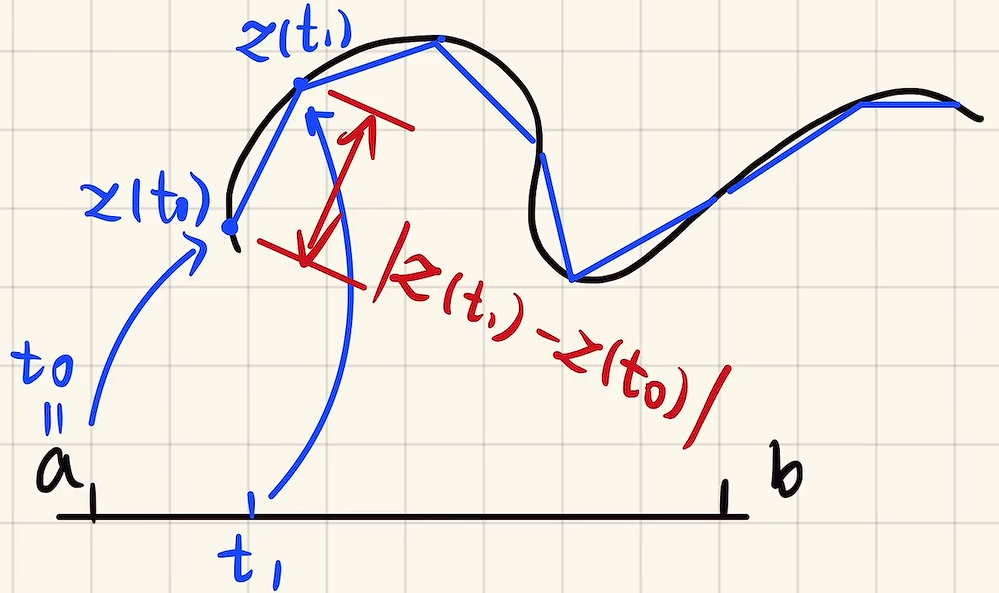
\includegraphics[width=0.4\linewidth]{figure/4.4.1-1}
			\caption{rectifiable curve}
			\label{pic : 4.4.1-1} % 添加图像引用标签
		\end{figure}
		
		\begin{rmk}
			为了表述的方便,后续我们常将$z$ 的值域视作复平面,即$z(t) = x(t) + iy(t)$.
		\end{rmk}
	\end{defn}

	\vspace{2em}
	在定义了曲线\textbf{可求长}的概念后,我们自然要问,在什么情况下\textbf{曲线可求长}? 即
	\begin{center}
		What condition on $x(t)$ and $y(t)$ guarantees rectifiability of $\gamma$?
	\end{center}
	为了解决这个问题,下面我们给出\textbf{有界变差函数}的定义,并会在后续给出这个问题的\textbf{充要条件},即
	\begin{center}
		$\gamma$ rectifiable $\,\, \Leftrightarrow \,\, x(t), y(t)$ 均为\textbf{有界变差函数}.
	\end{center}

\newpage
\paragraph{定义}
	下面给出\textbf{有界变差函数}的定义.
	\begin{defn}\label{def 4.4.2}
		Suppose $F : [a , b] \rightarrow \C$, and $\mathcal{P}$ is a partition $a = t_0 < t_1 < \cdots < t_N = b$. The \underline{\textcolor{blue}{\textbf{variation}}} of $F$ on this partition $\mathcal{P}$ is defined by
		\begin{align}
			V_{\mathcal{P}}(F) = \sum_{j = 1}^{N}{\left| F(t_j) - F(t_{j - 1}) \right|}
		\end{align}
		$F$ is said to be of \underline{\textcolor{blue}{\textbf{bounded variation (BV)}}} if $V_{\mathcal{P}}(F)$ is bounded over all partitions.
		
		\vspace{1em}
		
		\begin{rmk}
			\textbf{有界变差函数}不要求函数\textbf{连续},而在考虑\textbf{平面曲线}时默认函数\textbf{连续}.
		\end{rmk}
	\end{defn}

	\vspace{1em}
	下面就能够来回答\textbf{``引入"}中提到的问题,即\textbf{平面曲线可求长}的\textbf{充要条件}.
	\begin{thm}\label{thm 4.4.1}
		A curve parametrized by $F(t) = x(t) + iy(t)$, $a \leq t \leq b$, is rectifiable $\,\, \Leftrightarrow \,\,$ both $x(t)$ and $y(t)$ are of BV.
		
		\vspace{2em}
		\begin{proof}
			$\forall$ partition $\mathcal{P}$: $a = t_0 < t_1 < \cdots < t_N = b$, we have
			\begin{align}
				V_{\mathcal{P}}(F) = \sum_{j = 1}^{N}{\left| F(t_j) - F(t_{j - 1}) \right|}
			\end{align}
			Since $\left| a + bi \right| \leq \left| a \right| + \left| b \right| \leq 2 \left| a + bi \right|$,
			\begin{align}
				\left| F(t_j) - F(t_{j - 1}) \right| = \left| x(t_j) - x(t_{j - 1}) + i \left( y(t_j) - y(t_{j - 1}) \right) \right|
			\end{align}
			Then
			\begin{itemize}
				\item $\Leftarrow$: $\left| F(t_j) - F(t_{j - 1}) \right| \leq \left| x(t_j) - x(t_{j - 1}) \right| + \left| y(t_j) - y(t_{j - 1}) \right|$, then $\exists M < \infty$, $\st$
				\begin{align}
					V_{\mathcal{P}}(F) 
					&= \sum_{j = 1}^{N}{\left| F(t_j) - F(t_{j - 1}) \right|} \\
					&= \sum_{j = 1}^{N}{\left| x(t_j) - x(t_{j - 1}) \right|} + \sum_{j = 1}^{N}{\left| y(t_j) - y(t_{j - 1}) \right|} \\
					&\leq 2M , \,\, \forall partition \,\, \mathcal{P}
				\end{align}
				Therefore, the curve $F(t) = x(t) + iy(t)$ is rectifiable.
				
				\vspace{1em}
				
				\item $\Rightarrow$: $\left| x(t_j) - x(t_{j - 1}) \right| + \left| y(t_j) - y(t_{j - 1}) \right| \leq 2 \left| F(t_j) - F(t_{j - 1}) \right|$, then $\exists M < \infty$, $\st$
				\begin{align}
					\sum_{j = 1}^{N}{\left| x(t_j) - x(t_{j - 1}) \right|} + \sum_{j = 1}^{N}{\left| y(t_j) - y(t_{j - 1}) \right|} 
					\leq 2 \sum_{j = 1}^{N}{\left| F(t_j) - F(t_{j - 1}) \right|} 
					= 2 V_{\mathcal{P}}(F) 
					\leq 2M
				\end{align}
				Therefore, both $x(t)$ and $y(t)$ are of BV.
			\end{itemize}
		\end{proof}
	\end{thm}

\newpage
\paragraph{例子}
	下面来给出一些\textbf{有界变差函数}的例子.
	\begin{example}\label{ex 4.4.2}
		\begin{itemize}
			\item $x , x^2$ is of BV on $[a , b]$, $\forall [a , b] \subset \R$.
			
			\vspace{4em}
			\begin{proof}
				$\forall$ partition $\mathcal{P}$: $a = x_0 < x_1 < \cdots < x_N = b$, since $x$ is strictly increasing, then
				\begin{align}
					V_{\mathcal{P}}(x) 
					= \sum_{j = 1}^{N}{\left| x_j - x_{j - 1} \right|}
					= \sum_{j = 1}^{N}{x_j - x_{j - 1}} 
					= b - a < \infty
				\end{align}
				Also for $x^2$, 
				\begin{align}
					V_{\mathcal{P}}(x^2) 
					= \sum_{j = 1}^{N}{\left| x_{j}^2 - x_{j - 1}^2 \right|}
					= \sum_{j = 1}^{N}{\left| x_j + x_{j - 1} \right| \left| x_j - x_{j - 1} \right|}
					\leq 2b \sum_{j = 1}^{N}{\left| x_j - x_{j - 1} \right|}
					= 2b(b - a) < \infty
				\end{align}
				Therefore, both $x$ and $x^2$ are of BV on $[a , b]$, $\forall [a , b] \subset \R$.
			\end{proof}
		
			\vspace{10em}
			
			\item If $F$ is real-valued, monotonic, and bounded, then $F$ is of BV.
			
			\vspace{4em}
			\begin{proof}
				$\forall$ partition $\mathcal{P}$: $a = t_0 < t_1 < \cdots < t_N = b$. \\
				Since $F$ is bounded, $\exists M < \infty$, $\st \left| F \right| \leq M$. 不妨设$F$ 单调递增,
				\begin{align}
					V_{\mathcal{P}}(F) 
					= \sum_{j = 1}^{N}{\left| F(t_j) - F(t_{j - 1}) \right|}
					= F(b) -F(a)
					\leq 2M , \,\, \forall partition \,\, \mathcal{P}
				\end{align}
				So $F$ is of BV.
			\end{proof}
		
			\newpage
			
			\item \textbf{(书\footnote{\textbf{《$Real \,\, Analysis -- Measure \,\, Theroy, \,\, Integration, \,\, \& \,\, Hilbert \,\, Spaces$》--- $Elias \,\, M. \,\, Stein$}} P147 Ex 11)}. \\
			If $a , b > 0$, let
			\begin{align}
				f(x) = 
				\begin{cases}
					x^{a} \sin{(x^{-b})} , \,\, 0 \leq x \leq 1 \\
					0 , \,\, x = 0
				\end{cases}
			\end{align}
			Then 
			\begin{center}
				$f$ is of BV in $[0 , 1]$ $\,\, \Leftrightarrow \,\, $ $a > b$
			\end{center}
		
			\vspace{2em}
			\begin{proof}
				\begin{itemize}
					\item 先来考虑简单情形,即$f(x) = \sin{\frac{1}{x}}$. \\
					根据直觉,随着$x \to 0^{+}$,$\sin{\frac{1}{x}}$ 的震荡越剧烈,当分划足够密时,其变差中应当会出现各项为1的无穷级数,从而发散. 下面取一个特殊分划进行证明. \\
					对于$\forall$ 奇数$k \in \N$, 取
					\begin{center}
						$\frac{1}{x_k} = 2k \pi + \frac{\pi}{2}$, $\frac{1}{x_{k + 1}} = 2k \pi + \pi$
					\end{center}
					于是
					\begin{align}
						V_{\mathcal{P}}(f) 
						= \sum_{j = 1}^{N}{\left| \sin{\frac{1}{x_j}} - \sin{\frac{1}{x_{j - 1}}} \right|}
						= \sum_{j = 1}^{N}{1}
						= N , \,\, which \,\ is \,\, related \,\, to \,\, \mathcal{P}
					\end{align}
					故$\forall M < \infty$,当分划$\mathcal{P}$ 足够密时,$V_{\mathcal{P}}(f) > M$. 故$f$ 非BV.
						
				\vspace{2em}
				
				\item 对于一般情况,下面先讨论一种特殊分划$\mathcal{P}$. 即 \textbf{(Monotonic Partition, 单调划分)}
				\begin{align}
					[\frac{1}{x_{4k + 1}^b} , \frac{1}{x_{4k + 2}^b}] = [2k\pi + \frac{\pi}{2}, 2k\pi + \pi] , \,\,
					[\frac{1}{x_{4k + 3}^b} , \frac{1}{x_{4k + 4}^b}] = [2k\pi + \frac{3\pi}{2} , 2k\pi + 2\pi]
				\end{align}
				则以上述第一种的$[x_{4k + 1} , x_{4k + 2}]$ 举例,
				\begin{align}
					\left| x_{k + 1}^{a} \sin{\frac{1}{x_{k + 1}^{b}}} - x_{k}^{a} \sin{\frac{1}{x_{k}^{b}}} \right|
					= \left| x_{k + 1}^{a} \sin{\frac{1}{x_{k + 1}^{b}}} \right|
					= \frac{1}{(2k\pi + \frac{\pi}{2})^{\frac{a}{b}}}
					= O(\frac{1}{k^{\frac{a}{b}}})
				\end{align}
				同理对于$[x_{4k + 2} , x_{4k + 3}] , [x_{4k + 3} , x_{4k + 4}]  ,[x_{4k + 4} , x_{4k + 5}]$,均可得到
				\begin{align}
					\left| x_{k + 1}^{a} \sin{\frac{1}{x_{k + 1}^{b}}} - x_{k}^{a} \sin{\frac{1}{x_{k}^{b}}} \right|
					= O(\frac{1}{k^{\frac{a}{b}}})
				\end{align}
				于是
				\begin{align}
					\sum_{k = 0}^{N}{\left| x_{k + 1}^{a} \sin{\frac{1}{x_{k + 1}^{b}}} - x_{k}^{a} \sin{\frac{1}{x_{k}^{b}}} \right|}
					= O\left( \sum_{k = 1}^{N}{\frac{1}{k^{\frac{a}{b}}}} \right)
				\end{align}
				根据\textbf{p-级数}$\overset{\infty}{\underset{n}{\sum}}{\frac{1}{n^p}}$ 的收敛性 (收敛 $\Leftrightarrow$ $p > 1$)可得,
				\begin{align}
					&\sum_{k = 0}^{N}{\left| x_{k + 1}^{a} \sin{\frac{1}{x_{k + 1}^{b}}} - x_{k}^{a} \sin{\frac{1}{x_{k}^{b}}} \right|} < \infty \\
					&\Leftrightarrow \,\, \frac{a}{b} > 1 \,\, \Leftrightarrow \,\, a > b
				\end{align}
				由于对于任一分划$\mathcal{P}$,有:
				\begin{center}
					\textbf{``加密分割,变差不减"}
				\end{center}
				因此对于$\forall$ 分割,我们可以在其中加入如上节点,其变差不减,但因为上述节点中,$\sin{\frac{1}{x^b}}$ 在每个区间$[x_k , x_{k + 1}]$均单调,所以在各区间$[x_k , x_{k + 1}]$ 中的变差可直接去除绝对值,并得到
				\begin{align}
					V_{\mathcal{P}}(f) = O\left( \sum_{k = 1}^{N}{\frac{1}{k^{\frac{a}{b}}}} \right)
				\end{align}
				于是
				\begin{center}
					$f$ is of BV $\,\, \Leftrightarrow \,\, \frac{a}{b} > 1 \,\, \Leftrightarrow \,\, a > b$
				\end{center}
				\end{itemize}
			\end{proof}
		\end{itemize}
	\end{example}

\newpage
\subsection{有界变差函数的刻画}
\paragraph{介绍}
	本小节将给出\textbf{有界变差函数}的一个刻画,即
	\begin{center}
		\textbf{任一有界变差函数可差分为两个有界递增函数之差}.
	\end{center}
	同时还将研究函数的\textbf{全变差}的\textbf{性质}. 而这一切都是为了后续研究\textbf{微积分基本定理}做准备.
	
\vspace{2em}
\paragraph{定义}
	回顾函数的\textbf{变差}的概念\textbf{(Def \ref{def 4.4.2})}. 在此基础上,我们下面给出\textbf{全变差}的定义.
	\begin{defn}\label{def 4.4.3}
		Suppose $f : [a , b] \rightarrow \C$. The \underline{\textcolor{blue}{\textbf{total variation}}} of $f$ on $[a , x]$ ($a \leq x \leq b$) is defined by
		\begin{align}
			V_{f}([a , x]) = \sup_{all \,\, partitions}{\sum_{j = 1}^{n}{\left| f(t_j) - f(t_{j - 1}) \right|}}
		\end{align}
		In particular, if $f$ is real-valued, i.e. $f : [a , b] \rightarrow \R$. Then the \underline{\textcolor{blue}{\textbf{positive variation}}} of $f$ on $[a , x]$ is
		\begin{align}
			P_{f}([a , x]) = \sup_{all \,\, partitions}{\sum_{(+)}{f(t_j) - f(t_{j - 1})}}
		\end{align}
		Also the \underline{\textcolor{blue}{\textbf{negative variation}}} of $f$ on $[a , x]$ is
		\begin{align}
			N_{f}([a , x]) = \sup_{all \,\, partitions}{\sum_{(-)}{- \left[ f(t_j) - f(t_{j - 1}) \right]}}
		\end{align}
	
		\vspace{1em}
		\begin{rmk}
			\begin{itemize}
				\item \textbf{全变差}对\textbf{任一复值函数}均可定义,而\textbf{正变差}和\textbf{负变差}则只对\textbf{实值函数}有定义. 在后续的讨论中基本默认$f$ 为\textbf{实值函数}.
				
				\vspace{1em}
				
				\item 下面对定义中的符号$(+)$ 和$(-)$ 进行说明,即
				\begin{align}
					(+) &\coloneqq \{ j \mid f(t_j) \geq f(t_{j - 1}) \} \\
					(-) &\coloneqq \{ j \mid f(t_j) \leq f(t_{j - 1}) \}
				\end{align}
			
				\vspace{1em}
				
				\item 常常将\textbf{全变差}$V_{f}([a , b])$ 简记为$V_{a}^{b}(f)$.
			\end{itemize}
		\end{rmk}
	\end{defn}

\newpage
\paragraph{有界变差函数的刻画}
	在刻画有界变差函数之前,先来给出一个引理. 它说明了对于\textbf{实值有界变差函数}$f$,其\textbf{全变差与正、负变差之间的关系},以及\textbf{$f$ 与正、负变差的关系}.
	\begin{lemma}\label{lemma 4.4.2}
		Suppose $f$ is real-valued and of BV on $[a , b]$. Then for all $x \in [a , b]$, we have
		\begin{center}
			$f(x) - f(a) = P_{f}([a , x]) - N_{f}([a , x])$
		\end{center}
		and
		\begin{center}
			$V_{f}([a , x]) = P_{f}([a , x]) + N_{f}([a , x])$
		\end{center}
	
		\vspace{4em}
		\begin{proof}
			\begin{itemize}
				\item $f(x) - f(a) = P_{f}([a , x]) - N_{f}([a , x])$: \\
				$\forall \epsilon > 0$, $\exists$ a partition $\mathcal{P}$: $a = t_0 < t_1 < \cdots < t_N = b$, $\st$
				\begin{align}
					\left| P_{f} - \sum_{(+)}{f(t_j) - f(t_{j - 1})} \right| \leq \epsilon \,\, and \,\, 
					\left| N_{f} - \sum_{(-)}{- \left[ f(t_j) - f(t_{j - 1}) \right]} \right| \leq \epsilon
				\end{align}
				Then
				\begin{align}
					-\epsilon + \sum_{(+)}{f(t_j) - f(t_{j - 1})}
					&\leq P_{f} 
					\leq \sum_{(+)}{f(t_j) - f(t_{j - 1})} + \epsilon \\
					-\epsilon + \sum_{(-)}{- \left[ f(t_j) - f(t_{j - 1}) \right]}
					&\leq N_{f} 
					\leq \sum_{(-)}{- \left[ f(t_j) - f(t_{j - 1}) \right]} + \epsilon
				\end{align}
				Since 
				\begin{align}
					f(x) - f(a) 
					= \left( \sum_{(+)}{f(t_j) - f(t_{j - 1})} \right) - \left( \sum_{(-)}{- \left[ f(t_j) - f(t_{j - 1}) \right]} \right)
				\end{align}
				Then
				\begin{align}
					&P_{f} - N_{f} \in \left[ f(x) - f(a) - 2\epsilon , f(x) - f(a) + 2\epsilon \right] \\
					&\Rightarrow \,\, \left| \left( P_{f} - N_{f} \right) - \left( f(x) - f(a) \right) \right| \leq 2\epsilon , \,\, \forall \epsilon > 0
				\end{align}
				Since $\epsilon$ is arbitrary, letting $\epsilon \to 0$, we get $f(x) - f(a) = P_{f} - N_{f}$.
				
				\newpage
				
				\item $V_{f}([a , x]) = P_{f}([a , x]) + N_{f}([a , x])$: \\
				$\forall$ partition $\mathcal{P}$: $a = t_0 < t_1 < \cdots < t_N = b$, $\st$
				\begin{align}
					V_{\mathcal{P}}(f) 
					= \sum_{j = 1}^{N}{\left| f(t_j) - f(t_{j - 1}) \right|}
					= \left( \sum_{(+)}{f(t_j) - f(t_{j - 1})} \right) + \left( \sum_{(-)}{-\left[ f(t_j) - f(t_{j - 1}) \right]} \right)
				\end{align}
			
				\vspace{1em}
				
				\begin{itemize}
					\item $V_{f}([a , x]) \leq P_{f}([a , x]) + N_{f}([a , x])$: \\
					分别对右侧两项取上确界 through all partitions, we have
					\begin{align}
						\sum_{j = 1}^{N}{\left| f(t_j) - f(t_{j - 1}) \right|}
						\leq P_{f}([a  ,x]) + N_{f}([a , x])
					\end{align}
					再对左侧取上确界 through all partitions, then
					\begin{align}
						V_{f}([a , x]) \leq P_{f}([a , x]) + N_{f}([a , x])
					\end{align}
				
					\vspace{1em}
				
					\item $P_{f}([a , x]) + N_{f}([a , x]) \leq V_{f}([a , x])$: \\
					Similarly, 先对左侧取上确界,再对右侧分别取上确界,得到
					\begin{align}
						P_{f}([a , x]) + N_{f}([a , x]) \leq V_{f}([a , x])
					\end{align}
				\end{itemize}
			
				\vspace{1em}
			
				综上,$V_{f}([a , x]) = P_{f}([a , x]) + N_{f}([a , x])$.
			\end{itemize}
		\end{proof}
	\end{lemma}

	\newpage
	下面我们说明,\textbf{任一有界变差函数可差分为两个有界递增函数之差}.
	\begin{thm}\label{thm 4.4.3}
		A real-valued function $f : [a , b] \rightarrow \R$ on $[a , b]$ is of BV
		\begin{center}
			$\Leftrightarrow \,\,$ $f$ is the difference of two increasing bounded functions.
		\end{center}
	
		\vspace{4em}
		\begin{proof}
			\begin{itemize}
				\item $\Leftarrow$: Suppose $f = f_1 - f_2$, where $f_j$ is increasing and bounded on $[a , b]$, $j = 1 , 2$. \\
				Then by \textbf{Example \ref{ex 4.4.2}}, $f_j$ is of BV on $[a , b]$, $j = 1 , 2$. \\
				$\forall$ partition $\mathcal{P}$: $a=  t_0 < t_1 < \cdots < t_N = b$, since
				\begin{align}
					\left| f(t_j) - f(t_{j - 1}) \right| 
					\leq \left| f_{1}(t_j) - f_{1}(t_{j - 1}) \right| + \left| f_{2}(t_j) - f_{2}(t_{j - 1}) \right| , \,\, \forall j - 1 \sim N
				\end{align}
				Then since both $f_1$ and $f_2$ are of BV, $\exists M < \infty$, $\st$
				\begin{align}
					\sum_{j = 1}^{N}{\left| f(t_j) - f(t_{j - 1}) \right|}
					\leq \sum_{j = 1}^{N}{\left| f_{1}(t_j) - f_{1}(t_{j - 1}) \right|} + \sum_{j = 1}^{N}{\left| f_{2}(t_j) - f_{2}(t_{j - 1}) \right|}
					\leq 2M
				\end{align}
				Therefore, $f$ is of BV on $[a , b]$.
				
				\vspace{2em}
				
				\item $\Rightarrow$: By \textbf{Lemma \ref{lemma 4.4.2}}, $f(x) - f(a) = P_{f}([a , x]) - N_{f}([a , x])$, $\forall x \in [a , b]$. \\
				It's trivial to show that $P_{f}([a , x])$ is increasing in $x$. \\
				Similarly, we get $N_{f}([a , x])$ is increasing in $x$. Therefore
				\begin{center}
					$f(x) = \left( P_{f}([a , x]) + f(a) \right) - N_{f}([a , x])$
				\end{center}
				where $P_{f}([a , x]) + f(a)$ and $N_{f}([a , x])$ are increasing and bounded.
			\end{itemize}
		\end{proof}
	\end{thm}

\newpage
\subsection{有界变差函数的全变差的性质}
	在本小节的最后,我们来讨论一下\textbf{实值有界变差函数的全变差的性质}.
	\begin{proposition}\label{prop 4.4.1}
		Let $f \in BV([a , b])$ and be real-valued. Then
		\begin{enumerate}
			\item [(\rmnum{1})] $\forall c \in (a , b)$, $V_{f}([a , b]) = V_{f}([a , c]) + V_{f}([c , b])$.
			
			\vspace{1em}
			
			\item[(\rmnum{2})] $V_{f}([a , x])$ and $U(x) = V_{f}([a , x]) - f(x)$ are both increasing in $x$ on $[a , b]$.
			
			\vspace{1em}
			
			\item[(\rmnum{3})] $V_{f}([a , x])$ is continuous at $x_0$ $\,\, \Leftrightarrow \,\,$ $f$ is continuous at $x_0$.
		\end{enumerate}
	
		\vspace{4em}
		\begin{proof}
			\begin{enumerate}
				\item[(\rmnum{1})] 不难证明, $\forall c \in (a,  b)$,
				\begin{align}
					V_{f}([a , b]) = \sup{\left[ \sum_{j = 1}^{k}{\left| f(t_j) - f(t_{j - 1}) \right|} + \sum_{j = k + 1}^{N}{\left| f(t_j) - f(t_{j - 1}) \right|} \right]}
				\end{align}
				The sup is taken over all partitions with $a = t_0 < t_1 < \cdots < t_k = c < \cdots < t_N = b$. \\
				Since
				\begin{align}
					\sum_{j = 0}^{N}{\left| f(t_j) - f(t_{j - 1}) \right|}
					= \sum_{j = 1}^{k}{\left| f(t_j) - f(t_{j - 1}) \right|} + \sum_{j = k + 1}^{N}{\left| f(t_j) - f(t_{j - 1}) \right|}
				\end{align}
				Then 先对左侧取上确界 over all partitions on $[a , b]$, we have
				\begin{align}
					V_{f}([a , b]) 
					\geq \sum_{j = 1}^{k}{\left| f(t_j) - f(t_{j - 1}) \right|} + \sum_{j = k + 1}^{N}{\left| f(t_j) - f(t_{j - 1}) \right|}
				\end{align}
				再对左侧两项分别取上确界 over all partitions on $[a , c]$ and $[c , b]$, we have
				\begin{align}
					V_{f}([a , b]) \geq V_{f}([a , c]) + V_{f}([c , b])
				\end{align}
				Similarly, 改变两侧取上确界次序,可得
				\begin{align}
					V_{f}([a , b]) \leq V_{f}([a , c]) + V_{f}([c , b])
				\end{align}
				Therefore, $V_{f}([a , b]) = V_{f}([a , c]) + V_{f}([c , b])$, $\forall c \in (a , b)$.
				
				\newpage
				
				\item[(\rmnum{2})] Since $P_{f}([a , x])$ and $N_{f}([a , x])$ are both increasing, then by \textbf{Lemma \ref{lemma 4.4.2}},
				\begin{center}
					$V_{f}([a , x]) = P_{f}([a , x]) + N_{f}([a , x])$ is increasing in $x$ on $[a , b]$.
				\end{center}
				$\forall x \geq y$, we have
				\begin{align}
					V(x) - V(y) 
					&= V_{f}([a , x]) - V_{f}([a , y]) \\
					&= V_{y}^{x}(f) 
					\geq \left| f(x) - f(y) \right| 
					\geq f(x) - f(y)
				\end{align}
				Therefore $V(x) - f(x) \geq V(y) - f(y)$, $\forall x \geq y$. i.e.
				\begin{center}
					$U(x) \geq U(y)$, $\forall x \geq y$
				\end{center}
			
				\vspace{4em}
				
				\item[(\rmnum{3})] 
				\begin{itemize}
					\item $\Rightarrow$: 根据\textbf{(\rmnum{2})}的证明过程 (式(4.111)), we get
					\begin{center}
						$\left| V(x) - V(y) \right| \geq V(x) - V(y) \geq \left| f(x) - f(y) \right|$, $\forall x , y \in [a , b]$
					\end{center}
					Suppose $V(x)$ is continuous at $x_0$, then $\forall \epsilon > 0$, $\exists \delta > 0$, $\st$
					\begin{center}
						$\left| f(x) - f(x_0) \right| \leq \left| V(x) - V(x_0) \right| \leq \epsilon$, $\forall \left| x - x_0 \right| < \delta$
					\end{center}
					Then $f(x)$ is continuous at $x_0$.
					
					\vspace{2em}
					
					\item $\Leftarrow$: Suppose $f(x)$ is continuous at $x_0$. Fix $\epsilon > 0$, then $\exists \delta_0 > 0$, $\st$
					\begin{center}
						$\left| f(x_0 + h) - f(x) \right| < \frac{\epsilon}{2}$, $\forall \left| h \right| < \delta_0$
					\end{center}
					It suffices to show
					\begin{center}
						$\left| V(x_0 + h) - V(x) \right| < \epsilon$, $\forall$ small $h$
					\end{center}
					
					\vspace{1em}
					
					考虑\textbf{全变差}$V_{a}^{x_0}(f)$ and $V_{x_0}^{b}(f)$, for fixed $\epsilon > 0$, $\exists$ partitions
					\begin{align}
						a &= t_0 < t_1 < \cdots < t_n = x_0 \\
						x_0 &= s_0 < s_1 < \cdots < s_m = b
					\end{align}
					$\st$
					\begin{align}
						\left| V_{f}([a , x_0]) - \sum_{j = 1}^{n}{\left| f(t_j) - f(t_{j - 1}) \right|} \right| 
						&< \frac{\epsilon}{2} \\
						\left| V_{f}([x_0 , b]) - \sum_{j = 1}^{m}{\left| f(s_j) - f(s_{j - 1}) \right|} \right| 
						&< \frac{\epsilon}{2}
					\end{align}
					Now update $h$ with $\left| h \right| < h_0 = \min{\left\{ \delta_0 , x_0 - t_{n - 1} , s_1 - x_0 \right\}}$. \\
					下面先对$h > 0$ 的情况讨论.
					\begin{align}
						V(x_0 + h) - V(x_0)
						&= V_{x_0}^{b}(f) - V_{x_0 + h}^{b}(f) \\
						&\leq \sum_{j = 1}^{m}{\left| f(t_j) - f(t_{j - 1}) \right|} + \frac{\epsilon}{2} - V_{x_0 + h}^{b}(f) \\
						&= \left| f(s_0) - f(s_1) \right| + \sum_{j = 2}^{m}{\left| f(t_j) - f(t_{j - 1}) \right|} + \frac{\epsilon}{2} - V_{x_0 + h}^{b}(f) \\
						&\leq \left| f(x_0 + h) - f(x_0) \right| + \left| f(s_1) - f(x_0 + h) \right| + \sum_{j = 2}^{m}{\left| f(t_j) - f(t_{j - 1}) \right|} + \frac{\epsilon}{2} - V_{x_0 + h}^{b}(f)
					\end{align}
					Since $x_0 + h < s_1 < \cdots < s_m = b$ is a partition of $[x_0 + h , b]$, then
					\begin{align}
						\left| f(s_1) - f(x_0 + h) \right| + \sum_{j = 2}^{m}{\left| f(t_j) - f(t_{j - 1}) \right|}
						\leq V_{x_0 + h}^{b}(f)
					\end{align}
					Therefore
					\begin{align}
						V(x_0 + h) - V(x_0)
						&\leq \left| f(x_0 + h) - f(x_0) \right| + \frac{\epsilon}{2} \\
						&< \frac{\epsilon}{2} + \frac{\epsilon}{2}
						= \epsilon , \,\, \forall \left| h \right| < h_0
					\end{align}
					Similarly, 对于$h < 0$ 的情况,我们可同样估计$V(x_0) - V(x_0 + h) = V_{a}^{x_0}(f) - V_{a}^{x_0 + h}(f)$, 从而得出结论. \\
					综上, $V(x)$ is continuous at $x_0$.
				\end{itemize}
			\end{enumerate}
		\end{proof}
	\end{proposition}




	%  ############################
	\ifx\allfiles\undefined
\end{document}
\fi